% Template article for preprint document class `elsart'
% with harvard style bibliographic references
% SP 2001/01/05

%\documentclass[doublespacing]{elsart}
\documentclass[12t]{article}

% Use the option doublespacing or reviewcopy to obtain double line spacing
% \documentclass[doublespacing]{elsart}

% the natbib package allows both number and author-year (Harvard)
% style referencing;
\usepackage{natbib}
\usepackage{amsmath}
\usepackage{amssymb}
\usepackage{graphicx}
\usepackage{fancyvrb}
\usepackage[usenames]{color}
\usepackage{ulem}
\usepackage{afterpage}
\usepackage{subfigure}
\usepackage[tablesfirst,nomarkers]{endfloat}
%\usepackage[tablesfirst]{endfloat}
%\usepackage{lineno}
\definecolor{ch}{rgb}{0,.03,.85}

\newcommand{\redso}[1]{\textcolor{red}{\sout{#1}}}
\newcommand{\remove}[1]{\textcolor{red}{\sout{#1}}}

\newcommand{\red}[1]{\textcolor{red}{\uline{#1}}}
\newcommand{\new}[1]{\red{#1}}

\newcommand{\newp}[1]{\new{[new paragraph] }}



 \textheight  = 225 mm
 \textwidth   = 170 mm
 \hoffset     =  -5 mm
 \voffset     = -23 mm
 \evensidemargin =  0 mm
 \oddsidemargin  =  0 mm


% if you use PostScript figures in your article
% use the graphics package for simple commands
% \usepackage{graphics}
% or use the graphicx package for more complicated commands
% \usepackage{graphicx}
% or use the epsfig package if you prefer to use the old commands
% \usepackage{epsfig}

% The amssymb package provides various useful mathematical symbols
\usepackage{amssymb}
%\usepackage{endfloat}



\renewcommand{\topfraction}{.85}
\renewcommand{\bottomfraction}{.7}
\renewcommand{\textfraction}{.15}
\renewcommand{\floatpagefraction}{.66}
\renewcommand{\dbltopfraction}{.66}
\renewcommand{\dblfloatpagefraction}{.66}
\setcounter{topnumber}{9}
\setcounter{bottomnumber}{9}
\setcounter{totalnumber}{20}
\setcounter{dbltopnumber}{9}

%% TMH DEFS
 \def \bfmpost{{\bf m_p}}
 \def \bfCmpost{{\bf C_{m_p}}}
 \def \dip{\beta}
 \def \prior{{\rho}}
 \def \post{{\sigma}}
 \def \phys{{\Delta}}

 \def \dm{(\bf d,\bf m)}

% DEFINITIONS
 \def \bfd{{\bf d}}
 \def \bfm{{\bf m}}
 \def \bfg{{\bf g}}
 \def \bfh{{\bf h}}
 \def \bfk{{\bf k}}
 \def \bfp{{\bf p}}
 \def \bfu{{\bf u}}
 \def \bfv{{\bf v}}
 \def \bfw{{\bf w}}
 \def \bfx{{\bf x}}
 \def \bfy{{\bf y}}
 \def \bfA{{\bf A}}
 \def \bfC{{\bf C}}
 \def \bfD{{\bf D}}
 \def \bfK{{\bf K}}
 \def \bfX{{\bf X}}
 \def \bfZ{{\bf Z}}
 \def \bfZe{{\bf Z^{^{*}}}}


 \def \rmd{{\rm d}}
 \def \rmm{{\rm m}}
 \def \rmn{{\rm n}}
 \def \rmg{{\rm g}}
 \def \rmk{{\rm k}}
 \def \rmp{{\rm p}}
 \def \rmu{{\rm u}}
 \def \rmv{{\rm v}}
 \def \rmx{{\rm x}}
 \def \rmy{{\rm y}}
 \def \rmw{{\rm w}}
 \def \rmA{{\rm A}}
 \def \rmC{{\rm C}}
 \def \rmR{{\rm R}}
 \def \rmCov{{\rm Cov}}
 \def \rmD{{\rm D}}
 \def \rmK{{\rm K}}
 \def \rmR{{\rm R}}
 \def \rmX{{\rm X}}
 \def \rmZ{{\rm Z}}
 \def \rmV{{\rm V}}
 \def \bflambda{\boldsymbol{\lambda}}
 \def \PointP{{\mathscr{P}}}
 \def \PointQ{{\mathscr{Q}}}
 \def \LinSpaceL{\boldsymbol{\mathsf{L}}}
 \def \calA{{\cal A}}
 \def \calD{{\cal D}}
 \def \calE{{\cal E}}
 \def \calF{{\cal F}}
 \def \calK{{\cal K}}
 \def \calM{{\cal M}}
 \def \calN{{\cal N}}
 \def \calS{{\cal S}}
 \def \calZ{{\cal Z}}

 \def \eqn{eqn. }
 \def \eqns{eqns. }

 \def \absval#1{\left| \ #1 \ \right|}
 \def \norm#1{\Vert \ #1 \ \Vert}

 \def \onehalf{{\frac{1}{2}}}

 \def \ccondtab{{\ttfamily create\_condtab}}
 \def \dfcondtab{{\ttfamily draw\_from\_condtab}}
% \def \visimprog{{\ttfamily VISIM}}
 \def \visimprog{{VISIM}}
 \def \dssimprog{{\ttfamily DSSIM}}
 \def \sgsimprog{{\ttfamily SGSIM}}

 \def \visim{{\ttfamily visim}}
 \def \dssim{{\ttfamily dssim}}
 \def \sgsim{{\ttfamily sgsim}}
 \def \etype{{E-type}}

 \def \krig{{\ttfamily krig}}
 \def \krigv{{\ttfamily krig\_volume}}
 \def \cdv{{\ttfamily cov\_data2vol}}
 \def \cvv{{\ttfamily cov\_vol2vol}}
 \def \rpath{{\ttfamily rayrand\_path}}
 \def \nhood{{\ttfamily nhoodvol}}





\title{VISIM\\user guide}


\author{Thomas Mejer Hansen and Klaus Mosegaard\\
Niels Bohr Institute, Juliane Mariesvej 28, 2100 K\o benhavn \O, Denmark\\
http://imgp.gfy.ku.dk tmh@gfy.ku.dk}


\begin{document}
\maketitle

\begin{abstract}
This is an accompanion to the paper by Hansen and Mosegaard (submitted), describing in more detail how to run VISIM.
\end{abstract}




\section{Running \visimprog}
\label{sec:running}
A parameter file, in GSLIB style, is used to control \visimprog. Table
\ref{tab:par} show an example of a visim parameter file. Some parts of
the parameter file, for example variogram specification, are identical
to several GSLIB programs and for these we refer to the GSLIB book for
details, Deutsch and Journel (1997). 
The entries in italics in Table \ref{tab:par} are specific for running \visimprog, and will be documented here.

A default parameter file, \texttt{visim.par} (Table \ref{tab:par}), is written to disc when
\visimprog~is run without a parameter file. The parameters given in this default parameter file is the parameters referred to as defaults in the following.

The first 4 lines are for comments, and have no effect on running \visimprog.

\subsection{Type of conditional simulation}
Line 5 specifies which data to condition to. [0] unconditional, [1]
condition to both data of point and volume support, [2] condition only
to data of point support and [3] condition only to data of volume support. 
[1] is the default choice.

By choosing [2] \visimprog~behaves like a traditional sgsim or dssim
code conditioning to data of point support only.

\subsection{Specifying data of point support}
Hard data of point support are given in lines 6 and 7. Line 6 contain
the name of file containing the conditioning data, formatted in ASCII
GSLIB format, also known as the EAS ASCII format. Each line in the
file described one hard data, and the columns for [x,y,z] location and the data
values are given in line 7.

\subsection{Specifying data of volume support}
Lines 8 and 9 contain the name of two files describing the geometry of
the weighting function for volume average data (\texttt{visim\_volgeom.eas}) and actual
observed data and uncertainty (\texttt{visim\_volobs.eas}). Both files
use the ASCII GSLIB format.

Note that the geometry of the volume average data can be completely
arbitrary, and volumes need not be coherent areas.

Table \ref{tab:volgeom} show a small part of an example of \texttt{visim\_volgeom.eas}. Each row defines one point, $\rmu$, within a data observation of volume support.
The first three columns specifies the [x,y,z]-location of points within volume support. 
 The fifth column indicate the weight, $\rmw(\bfu)$, of the point within the data of volume support as indicated by column four. 

Table \ref{tab:volobs} show a small part of an example of
\texttt{visim\_volobs.eas}. Each row contains information about one
data observation of volume support. The first columns simply list the
data number, the same as the fourth column in the
\texttt{visim\_volgeom.eas} file. The second column lists the number
of data within each data of volume support. This is mainly listed to
use as a consistency check between the two data files. The third and
fourth column contains the data observations and their associated uncorrelated uncertainties.

Thus,  \texttt{visim\_volgeom.eas} contains a description of the geometry of the weighing function of each observed data of volume support, and  \texttt{visim\_volobs.eas} contain the actual data observation and the measurement error.

Note that a data of point support with measurement error can be given as a volume average data sensitive to only one [x,y,z] location and with weight '1' (i.e. only one line in \texttt{visim\_volgeom.eas}), as well as the corresponding line in \texttt{visim\_volobs.eas} containing the data observation and measurement error.  

\subsection{Debug level}
The amount of verbose information written to the screen and to disk
files during simulation is controlled by the debug level as given in
line 11. When running \visimprog~to tune the input parameters for best
performance, a relative high debug level of 3 will ensure that most
information will be available. A higher debug level than 3 is only
needed when performing actual debugging of the source code.
A default debug level of -1 is suggested when running \visimprog~in
production mode.

\subsection{Reading covariance lookup table from disk}
The second flag of line 11 (read\_covtab) controls whether the covariance table should be read from disk. If set to one [read\_covtab=1] they are read from the files cv2v\_parfile.out and cd2v\_parfile.out. Both of these files are binary ( 64 bit floating point ) sequential Fortran files.

The files cv2v\_parfile.out and cd2v\_parfile.out are always generated at the end of a visimprog~run if the debug level is above -1.

In case read\_covtab is set to 1, but the covariance files does not exist, a warning will be written to screen, and \visimprog~will progress as if read\_covtab=0.
 

\subsection{Reading 'lambda' from disk}
The third flag of line 11 controls whether the kriging weights are actually computed ([0] default) or read from disk [1] (from file lambda\_parfile.out).

When read\_lambda=0, \visimprog~behave like a traditional kriging/simulation algorithm. I.e. the kriging weights of the kriging system are found using matrix inversion. In this mode, kriging weights are written to disk, in the file lambda\_parfile.out

When read\_lambda=1 no kriging system is in fact inverted, and the kriging weights are simply loaded from disk. This is useful in cases where one have the same data geometry (this includes uncertainty on data, not just location in space). Then the same sets of weights can be used for different data sets.

In case read\_lambda=-1 no lambda data are written to disk.


\subsection{Output}
Estimation or simulation output are saved to the filename listed in line 12. In addition any verbose information, as for example the covariance lookup tables, are saved to various filenames (indicating the content) with the output filename appended. Thus from one run of \visimprog, a number of files are created, all ending with the text string as given by the filename in line 12.

\subsection{Number of realizations}
Line 13 indicates the number of realizations to generate when using \visimprog. If this is selected as '0' (zero), then estimation is performed, rather than simulation. This means that the kriging mean and variance are output in the file specified in line 15. Thus, no values are drawn from the local conditional probability density functions, and therefore no values are added to the list of previously simulated point data.

Performing estimation can be handy for several reasons. For example
the result of running
\visimprog~in sgsim estimation mode, with infinitely large data
neighborhoods, is strictly identical to the 
solution obtained using least squares based linear inversion, Tarantola (2005, page 66).
Also, the E-type mean, point-wise mean of all generated simulations in
simulation mode,
is identical to the kriging obtained running kriging in estimation
mode, given infinitely many realizations. 

Because of the analogue to least squares linear inversion
\visimprog~can be used to solve weakly non-linear inverse problems,
i.e. non-linear problems that can be linearized around a prior model.
A weakly non-linear inverse problems can be solved in an iterative
manner by solving a linear inverse problem in each iteration, Tarantola (2005).
Thus \visimprog~can be used in each iterative step to solve the linear
inverse problem running in estimation mode.
In the last iterative step of the inversion one can perform simulation
rather that estimation to obtain samples of the a posteriori
distribution of the weakly non-linear problem.

\subsection{Reference distribution}
The choice of sgsim or dssim is selected in line 14.
[0] selects sgsim (default) and [1] selects dssim.


\subsubsection{dssim - histogram reproduction}
When dssim [1] has been selected, a number of options are available for controlling histogram reproduction.

The target histogram to match is computed from the list of data input through the file defined in line 15, \texttt{reference.eas}, which is an ASCII formatted EAS file.

Lines 17-18 controls the range and number of mean and variance values
in normal score space to back transform into a lookup table. Width a
wider range and the more samples, the histogram reproduction will be
better.
By default 100 mean values between -3.5 and 3.5, and 100 variance
values between 0 and 1.2 are selected.
Line 19 set the number of quantiles to back transform from normal
score space (\texttt{n\_q}).
By default these are set to  \texttt{n\_q}=170.
As the case study will show, these options should be carefully chosen to ensure optimal results.

The mean and variance of the back transformed distributions are saved
on disk to the files \texttt{cond\_mean\_visim.out} and 
\texttt{cond\_var\_visim.out}.
The kriging mean and variance calculated at each grid node is
saved to the file 
\texttt{krig\_visim.out} only if the debug level is set to 2 or higher.
As suggested by \cite{Deutsch:2000:DSSIM-HR} these three files can be used to check if the back transformed
means and variances span the range needed by kriging, as we shall
investigate in practice later.
The back transformed distributions, associated to the back transformed
mean and variance, is saved to the file 
\texttt{cond\_cpdf\_visim.out}
if the debug level is chosen to 3 or higher.

Lines 36-38 control the behavior of the normal score transform for the
head and tail of the reference distribution and follow the GSLIB style described by Deutsch and Journel (1998, page 135).
\texttt{z\_min} and \texttt{z\_max}, the choices of minimum and
maximum value used for extrapolation, line 36, are critical for obtaining good
realizations. These must be chosen carefully and consistent with the choice of
target distribution.
The choice of type of interpolation for the upper and lower tail, lines
37-38, is less significant, and can in general be left at default
values.

In summary, lines 15,17-19,36-38 are only used when dssim is chosen,
otherwise they are ignored. When dssim is chosen one can in general
use the default values affecting dssim, except that upper and lower
limit, \texttt{z\_min} and \texttt{z\_max} in line 36, must be chosen
carefully, as well as the parameters of lines 17-18. 

\subsection{Volume average neighborhood selection} 
The three parameters in line 26, (\texttt{method,nvol,
  accept\_fraction}), control the volume average neighborhood. 
The first option, \texttt{method}, denotes the type of
neighborhood. The two latter options are used to control aspect of the
neighborhood depending on the neighborhood type selected. 
The second option, \texttt{nvol}, denotes a number of volume average
data, and \texttt{accept\_fraction} is a relative threshold covariance
value with respect to the global variance. If the global variance
(defined at line 32) is set to .2, a choice of  
\texttt{accept\_fraction}=0.1, refers to a covariance threshold of $0.02$. 

\texttt{method} takes the values 0,1,2 and 3[default]:
[0] All volume average data is used all the time. This can become quite CPU demanding.
[1] Only volume average data with a covariance to the point being
simulated above the threshold as indicated by
\texttt{accept\_fraction} is used. 
[2] As [1], but use a maximum of \texttt{nvol} volume average data.
[3] Use exactly \texttt{nvol} volume average data. The volume average data with the highest covariance to the point being simulated is chosen.

\subsection{Choice of random path} 
Three types of random paths, all previously discussed, can be selected in line 27. [0] Independent random path, [1] 'Volumes-first' random path and [2] preferential random path. 


\subsection{visimprog~in dssim mode}
To use \visimprog~ in dssim mode one must provide the target
histogram to match. If the target distribution is relatively close to
a Gaussian distribution, the given default parameters for histogram reproduction, as presented
earlier, will provide realizations which honor the a priori statistics. 
However if the target distribution is far from Gaussian one may need
to revisit the options for setting up the lookup table for the local
distribution, with associated mean and variance. We will therefore shortly illustrate the effect of using specific parameters for controlling histogram reproduction.

As pointed out by Deutsch (2000), one does not have detailed control
over for which sets of local mean and variance the local conditional lookup
table is calculated. Even if one selects a extremely dense sampling of
the mean and variance in normal score space, the distribution in
back-transformed space may not show the range of local mean and variance needed. 

Therefore one can check, as suggested by Deutch (2000), how well the computed local mean and
variances, found in the files \texttt{cond\_mean\_visim.out} and 
\texttt{cond\_var\_visim.out}.
cover the kriging mean and variance, that are returned from the local
kriging, as found in the file \texttt{krig\_visim.out}.

Consider first, for comparison, reference target data set consisting of  30000 samples
from a Gaussian distribution with mean of 0.13, and a variance of
0.0002. This is the distributions shown as a black dashed line in Figure \ref{fig:dssim_covlookup_coverage}a  


Using default parameters for histogram reproduction,
Figure \ref{fig:dssim_covlookup_coverage}a show the cross plot of the mean and variance of the back
transformed local pdf, black dots,
as located in the local pdf lookup table using the Gaussian target distribution. Also plotted is the cross plot of the actual estimated kriging mean and variances, white dots, as
computed through sequential simulation. 
Deutsch points out two critical features highlighted by this cross plot. First the distance from any white dot (the kriging mean and variance) to the nearest black dot (the closest set of local mean and variance in the lookup table) must not be too large. Second, and most importantly, all kriging mean and variance values (white dots) should be located within the cloud spanned by the local mean and variance values of the lookup table (black dots). If not, one is likely to select a wrong local conditional distribution to draw a value from during simulation.

Using a Gaussian distributions as target distribution, Figure
\ref{fig:dssim_covlookup_coverage}a clearly shows that the white dots
are well covered by black dots. The histogram of 100 unconditional
simulations shown in Figure \ref{fig:dssim_covlookup_coverage}a and the corresponding variation of the experimental semivariogram, Figure \ref{fig:dssim_uncond_semivar}a, show nice reproduction of both the mean, variance, histogram and semivariogram. The tendency of a slightly lower sill value (averaging at 1.9e-4) of the experimental semivariogram than that of the a priori semivariogram(2.0e-4), is also noted by Robertson et al., (2006). 

Next we consider a bimodal target distribution, given by the dashed
line of Figure \ref{fig:dssim_covlookup_coverage}b and once again we
use the default values for histogram reproduction. A bimodal
distribution is selected as Deutch (2000) reported that honoring the target histogram using dssim was most difficult using distributions far from Gaussian. In this way we aim to check the limits of accuracy of dssim histogram reproduction.
First of all Figure \ref{fig:dssim_covlookup_coverage}b show that many sets of kriging mean and variance is located outside the cloud of local kriging mean and variance values. In addition the distribution of local kriging mean and variance values is much more focused on specific areas, and for example local mean values around 0.13 with a low variance is relatively poorly represented. 

The result of running 100 unconditional realizations result in the
histogram and experimental semivariogram as given in Figure
\ref{fig:dssim_covlookup_coverage}b and \ref{fig:dssim_uncond_semivar}b. The shape of the target histogram is picked up by all realization, though there is a tendency to slight smoothing. The experimental semivariogram, Figure \ref{fig:dssim_uncond_semivar}b, show the right shape, but again the sill values varies around 1.92e-4, which is a bit lower than chosen a priori chosen.

Finally consider the same bimodal model as considered above but using a wider and denser choice of samples parameters in normal score space.
We choose to consider mean values in normal score space ranging from -5 to 5, and 300
variance values in normal score space, ranging from 0 to 1.3. This
result in the cross plot of the mean and variance of the back transformed
local probability density functions in the lookup table, as shown in
Figure \ref{fig:dssim_covlookup_coverage}c. 
Compared to Figure \ref{fig:dssim_covlookup_coverage}b it is clear that the kriging mean and variance are much better covered by the available sets of local mean and variance values, than when using the default parameters for histogram reproduction.
The result of running unconditional simulation show a histogram that
looks much like when using the default parameters, Figure
\ref{fig:dssim_covlookup_coverage}c, still not picking up the highest
frequency variation of the target histogram, but still obtaining most
of the shape of the target histogram.
The sill value of the experimental semivariogram (0.00020) is
reproduce the a priori chosen sill value nicely, Figure \ref{fig:dssim_uncond_semivar}c.

Using the found set of parameters for controlling the histogram reproduction, conditional simulation is considered. 
Figure \ref{fig:dssim_conditional}a show seven conditional
realizations and the E-type for all 100 realizations, that all contain the main features of the reference model, Figure \ref{fig:refmodel}b, 

The experimental 
semivariogram of the 100 realizations tend to vary nicely around the
semivariogram model of the reference model,  Figure \ref{fig:dssim_conditional}a, and the histogram also
matches that of the reference model very well,  Figure \ref{fig:dssim_conditional}c 

The observed variance of the distribution of data misfit, 4.3e-6, for
all rays and all realizations, Figure \ref{fig:dssim_conditional}d, matches the chosen
variance of measurement error (4e-6) quite well.

Considering that the chosen bimodal target histogram, is one of the of the more difficult distributions to match in dssim mode as compared to more Gaussian like distributions, the results
clearly that \visimprog~can be used in dssim mode to draw samples of
the a posteriori probability function of a non-Gaussian linear inverse
problems. 


\section{Weakly non-linear linear inverse problems}
The straight approach is adopted for the previous tomography examples. In reality, this is only true in case there is no velocity contrast (as in for example CAT scan tomography). In cross borehole experiments the velocity contrasts will typically be so large that the straight ray approximation will not be appropriate. However, assuming non-straight rays, the inverse tomography problems becomes non-linear: the propagating ray path (the linear averaging kernel) depend on the velocity model, which is unknown.
In practice cross borehole tomography can be treated as a 'weakly' non-linear problem.  By a 'weakly' non-linear problem we refer to a non-linear problem that can be linearized around some model (Tarantola, 2005). Hansen et al. (2006) suggest how a combination of estimation and simulation can be used to solve such weakly non-linear problems. This is what we will demonstrate here.

In the examples used previously we also make use of the high frequency approximation to the wave equation, i.e. only the shortest length ray path is considered. In reality wave propagation is band-limited, and thus, the arrival time is a function of an averaging kernel around the ray path, \cite{Woodward}. 
We will also show how such linear average kernels can be easily included in \visimprog.

We consider again the reference model of Figure  \ref{fig:refmodel}a. Using a source frequency of 125 MHz we compute the linear average kernel associated with the reference model. 
The shape of this averaging kernel can be efficiently computed using calculation of first arrival fields as described by for example \cite{Munk}. 
Figure \ref{fig:true_nonlin_kernel} show the linear average kernel as computed from a 
constant velocity model (\ref{fig:true_nonlin_kernel}a), 
the true velocity (\ref{fig:true_nonlin_kernel}b), and a detailed look at the averaging kernel for 12 propagating waves (\ref{fig:true_nonlin_kernel}c).  As can be seen the kernel of the straight ray approximation differs considerably from the true kernel.

Using the true averaging kernel we calculate a set of observed data, $\bfd$, to which we add Gaussian uncorrelated noise with mean 0 and variance 4e-6. This is now our reference data set.

This linear average kernel is off course unknown prior to inversion. A realistic scenario is to a priori assume a constant velocity field with mean 0.13, and a frequency of 125 MHz of the source wavelet. This result in an initial linear average (for which the center of the averaging kernel is straight lines) as illustrated in Figure \ref{fig:true_nonlin_kernel}a.

As given by Hansen et al. (2006) the weakly non-linear tomography inversion problem may now be linearized as follows: 
From a starting velocity model, Vold, a linear average kernel is calculated as given above. Using this current kernel, sequential estimation is used to calculate the center of the posterior Gaussian pdf (ie. the kriging mean). This is labeled Vnew. We then select a current velocity model, Vc, as the sum of the old model and a proportion,$d$,  of the change given by the new model, such that Vc=Vc+$d$(Vnew-Vc). If the change in background velocity model (Vnew-Vc) is large (this is subjectively chosen) the iteration continues such that Vc=Vnew.
At each step the appropriate averaging kernel is computed from the current velocity model, Vc. After some iterations (in this case 5) there is little to no change between Vc and Vnew. 
If the inverse problem is properly linearized then the found linearized linear average kernel should reflect the true kernel. If this is not the case, then this method of linearization cannot be used, and more general non-linear inversion should be considered.


Figure \ref{fig:iterative_kernel} show how the averaging kernel change. The area of high sensitivity (black region) is gradually moved to the center of the model, while the area above and below this high sensitivity area is depleted of sensitivity.
The linear average kernel found using the iterative linearization process (Figure \ref{fig:iterative_kernel}, itearation 5), is quite close to the true kernel, Figure \ref{fig:iterative_kernel}, right.

Figure \ref{fig:iterative_sim} compare samples of the a posteriori pdf using the true kernel (top), a 'linear' kernel (based on a constant velocity field) (middle) and the linearized kernel (bottom) found through the iterative process. In all cases the high velocity zone in the middle of the model is clearly outlined. However the dipping low velocity layers above and below the high velocity area in the middle of the model are badly resolved using the linear kernel. Specifically, the low velocity layer dipping from a depth of 2m to the left in the model to a depth of 3-4m in the right side of the model, does not seem to be connected across the model using the linear kernel. This is contrary to using the true and the linearized kernel. 
Such artifacts can have severe implications if samples of the posterior are to be fed to for example a flow modeling engine. Then such non-connected layers, where it is really connected, can have major impact on modeling results.


This type of linearization is only valid for weakly non-linear problems, or in cases when ones starting model, and hence initial averaging kernel, is close to the true one. If this is not the case one may not locate the true averaging kernel, and the use of linear theory (and the simple kriging system) is invalid.

In the present case the non-linear inverse problems could clearly be linearized using the suggested iterative approach.
\vspace{1cm}

\section{Conclusion}
\label{sec:conclusion}

\textbf{Acknowledgement}
We thank Albert Tarantola and Andre Journel for concise discussion on the similarities of linear inverse theory and geostatistics, and in general for great discussion. We thank Yongshe Liu for guidance into GSLIB. Majken Looms is acknowledged for providing a cross bore hole setup geometry. The geostatistical Matlab toolbox, mGstat (http://mgstat.sourceforge.net/), can be used to run, control and visualize the output of \visimprog.


\nocite{Robertson:2006:DSSIM}
\nocite{Soares:2001:DSS}
\nocite{Oz:2003:DSSIM-HR}
\nocite{Journel:1978:MG}
\nocite{Journel:1999:VOL}
\nocite{Goovaerts:1997}
\nocite{Soares:2001:DSS}
\nocite{Oz:2003:DSSIM-HR}
\nocite{Deutsch:2000:DSSIM-HR}
\nocite{GSLIB}
%\nocite{Journel:1993:MU}
\nocite{Hansen:2006:geostatinv}
\nocite{Liu:2006:FFTcov}

\nocite{SrinavasanJournel:1998}
\nocite{GomezHernandez:2000:CapeTown}
\nocite{GomezHernandez:2004:Banff}

\nocite{Gloaguen:2005}
\nocite{Gloaguen:2004:Banff}

\bibliographystyle{elsart-harv}
\bibliography{../../LATEX/bibtex/thomas}                     

\clearpage
\begin{table}
\scriptsize
\begin{Verbatim}[fontfamily=tt,numbers=left,commandchars=\\\{\}]
                  Parameters for VISIM
                  ********************

START OF PARAMETERS:
1                             - conditional simulation (0=no,1:(p,v), 2:(p), 3:(v)
visim_cond.eas      - file with conditioning data
1  2 3 4                      - columns1 for X,Y,Z,val
\textit{\textcolor{ch}{visim_volgeom.eas            -  Geometry of volume/ray}}
\textit{\textcolor{ch}{visim_volobs.eas              -  Summary of volgeom.eas.}}
-1.0       1.0e21             -  trimming limits for conditioning data
-1 0 -1                            -debugging level: 0,1,2,3, read\_covtab [1=from disk], read\_lambda
visim_iso.out                     -file for output
\textit{\textcolor{ch}{10                       -number of realizations to generate}}
\textit{\textcolor{ch}{1                             -ccdf. type: 0-Gaussian, 1-Dssim-histogram reproduction}}
reference.eas            - reference histogram
1    0                        - columns for variable and weights
\textit{\textcolor{ch}{-3.5   3.5  100               - min_Gmean, max_Gmean, n_Gmean}}
\textit{\textcolor{ch}{0      2    100               - min_Gvar, max_Gvar, n_Gvar}}
\textit{\textcolor{ch}{170                           - n_q, n_Gsim}}
21    .125    .250             -nx,xmn,xsiz
49    .125    .250              -ny,ymn,ysiz
1     .125    .250              -nz,zmn,zsiz
69067                         -random number seed
0     8                       -min and max original data for sim
28                            -number of simulated nodes to use
\textit{\textcolor{ch}{3 32 0.001                         -Volume Neighborhood, method[0,1,2] , nusevols, accept_frac}}
\textit{\textcolor{ch}{0                          -Random Path, [1] independent, [2] rays first, [3] preferential}}
1                             -assign data to nodes (0=no, 1=yes)
0                             -maximum data per octant (0=not used)
3.6000  3.6000  2.6000              -maximum search radii (hmax,hmin,vert)
 0.0   0.0   0.0              -angles for search ellipsoid
.1304 0.0002                      - global mean and variance
1    .000000                 -nst, nugget effect
1    0.0002  83.5.0   0.0   0.0     -it,cc,ang1,ang2,ang3
      4.0  1.0  1.0      -a_hmax, a_hmin, a_vert
\textit{\textcolor{ch}{4.2   5.8                          - zmin,zmax (tail extrapolation for target histogram)}}
\textit{\textcolor{ch}{1      -5.4                   -  lower tail option, parameter}}
\textit{\textcolor{ch}{1      6.3                   -  upper tail option, parameter}}
\end{Verbatim}
\caption{Input parameter file for \visimprog.}
\label{tab:par}
\end{table}


\clearpage
\begin{table}
\begin{Verbatim}
Geometry of volume support data
5
X center of node.
Y center of node.
Z center of node.
Data number.
Weight of each point within Data
   1.4375      0.4875      0.0125         2   0.0166667
   1.4625      0.4875      0.0125         2   0.00833333
   1.4625      0.5125      0.0125         2   0.00833333
   1.4875      0.5125      0.0125         2   0.0166667
   0.0125      0.0125      0.0125         3      0.0125
   0.0125      0.0375      0.0125         3   0.00416667
   0.0375      0.0375      0.0125         3   0.0166667
   0.0625      0.0375      0.0125         3   0.00416667
   0.0625      0.0625      0.0125         3      0.0125
   0.0875      0.0625      0.0125         3      0.0125
   0.0875      0.0875      0.0125         3   0.00416667
\end{Verbatim}
$\vdots$
\caption{\visimprog~ Geometry of data of volume support}
\label{tab:volgeom}
\end{table}


\clearpage
\begin{table}
%\scriptsize
\begin{Verbatim}
Observations of data of volume support
4
Data number
Number of points in data
weighted average data observation
uncertainty of weighted average data observation
          1            60       5.13668        0.01
          2            80       5.10377        0.01
          3           100       5.02879        0.01
...
\end{Verbatim}
\caption{\visimprog~ Measurements of data of volume support}
\label{tab:volobs}
\end{table}

%\input{visim_CandG_submit_figures_format}


%clearpage
\begin{figure}
  \centering
  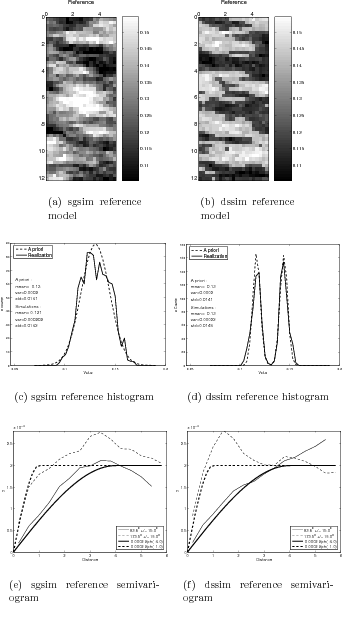
\includegraphics{fig_3}

  \caption[Reference velocity model for a) sgsim and b) dssim and the histigrogram for each velocity model below.]{}
\label{fig:refmodel}
\end{figure}



\clearpage
\begin{figure}
  \centering
  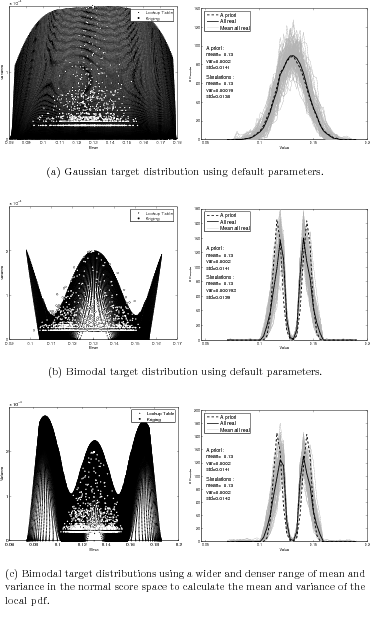
\includegraphics{manfig_13}

  \caption[Left) Comparison of the the mean and variance of the local lookup table (black dots) compared to the actual kriging mean and variances (white dots).
Right) Histogram computed from 100 realizations compared to the target distribution and the mean of all 100 histograms.
]{}
\label{fig:dssim_covlookup_coverage}
\end{figure}
 

\clearpage
\begin{figure}
  \centering
  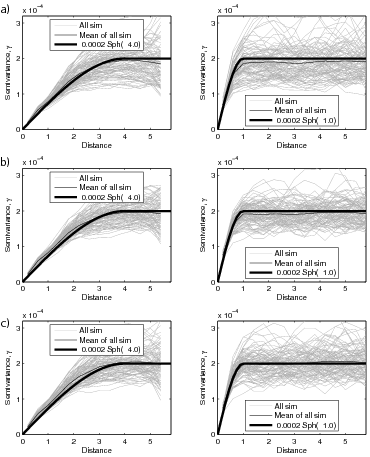
\includegraphics{manfig_14}
  \caption[Experimental semivariograms of 100 unconditional realizations using the target histogram properties as given in Figure \ref{fig:dssim_covlookup_coverage}. 
top) Gaussian target histogram.
middle) bimodal target histogram.
bottom) bimodal target histogram using a wider and more densely sampling of mean and variances in normal score space.
]{}
\label{fig:dssim_uncond_semivar}
\end{figure}



% FIGURE 7
%%%
%%% DSSIM EXAMPLE
%clearpage
\begin{figure}
\centering
  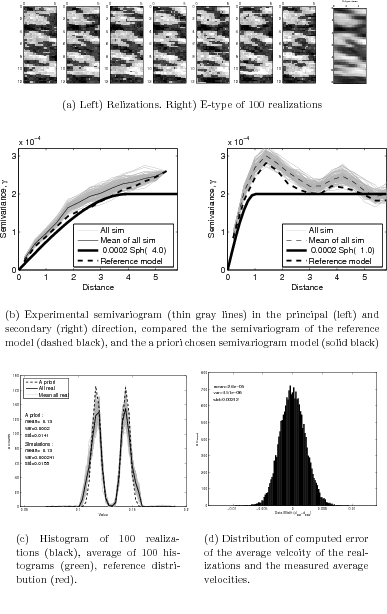
\includegraphics{manfig_7}
%  \includegraphics{fig_15}
%\subfigure[Left) Relizations. Right) E-type of 100 realizations]{\includegraphics[height=3cm]{dssim_cond_3_sim}\quad
%                    \includegraphics[height=3cm]{dssim_cond_3_etype}}\\
%\subfigure[Experimental semivariogram (thin gray lines) in the principal (left) and
%secondary (right) direction, compared the the semivariogram of
%the reference model (dashed black), and the a priori chosen semivariogram model
%(solid black)]{\includegraphics[width=\textwidth]{visim_dssim_semivar_compare_2}}\\
%\subfigure[Histogram of 100 realizations (black), average of 100
%histograms (green), reference distribution (red).]{\includegraphics[angle=-0,width=6.5cm]{dssim_cond_3_stat}}
%\subfigure[Distribution of computed error of the average velcoity of the realizations and the measured average
%velocities.]{\includegraphics[angle=-0,width=6.5cm]{dssim_cond_3_volfit}}
\caption[dssim conditional simulation]{}
\label{fig:dssim_conditional}
\end{figure}


\begin{figure}
\centering
%  \includegraphics{fig_8}
  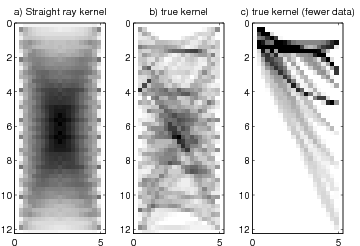
\includegraphics[width=14cm]{true_nonlin_kernel_color}
\caption[Linear averaging kernels using a) a constant velocity field,  b) the true velocity field, and c) as a) but only for 12 propagating wavefields. White indicate low sensitivity (ie. little weight in the averaging kernel) and black high sensitivity.]{}
\label{fig:true_nonlin_kernel}
\end{figure}




% FIGURE 9
\begin{figure}
\centering
%  \includegraphics{fig_9}
  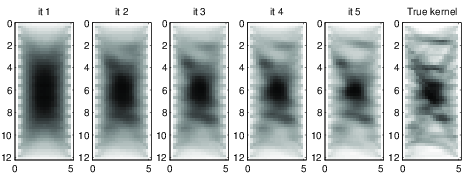
\includegraphics[width=14cm]{iterative_kernel_f2_color}
\caption[The evolution of the kernels sensitivity density in 5 iterative steps. right) the true kernel for comparison. Black reflects high and white low sensitivity]{}
\label{fig:iterative_kernel}
\end{figure}


% FIGURE 10
\begin{figure}
\centering
  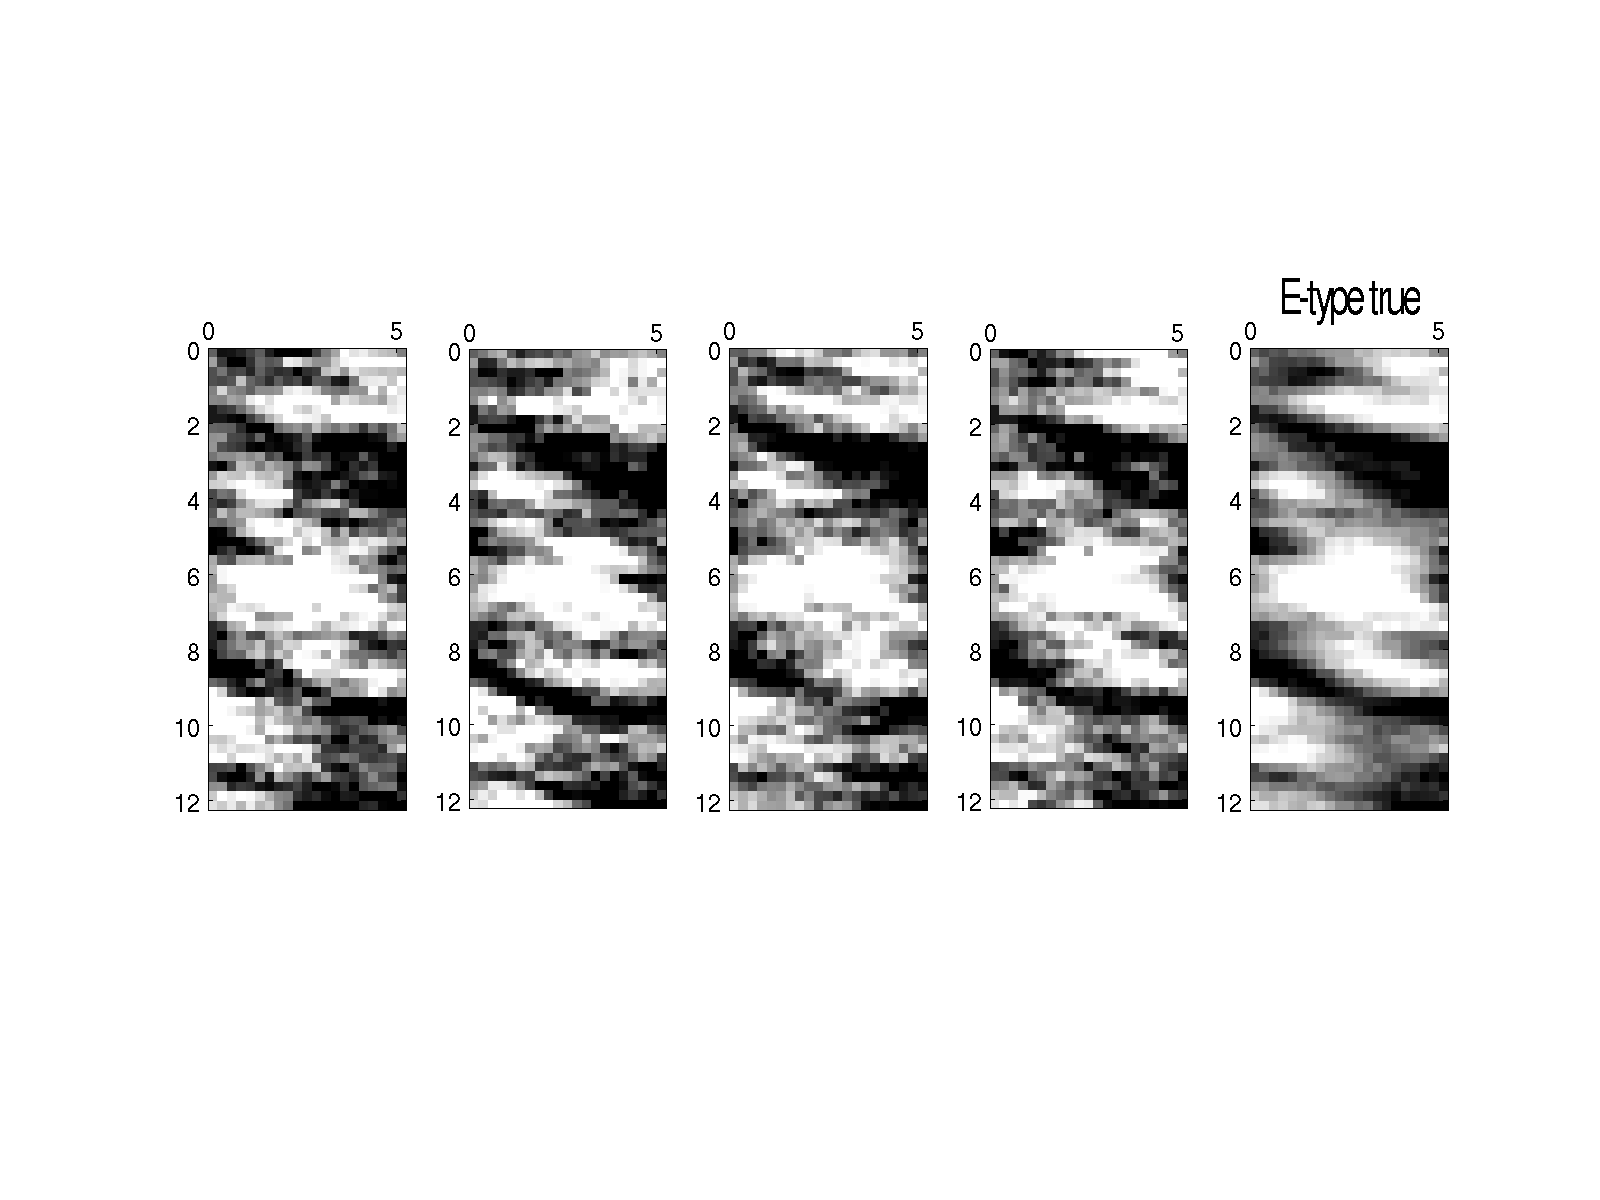
\includegraphics[width=14cm]{sim_true}
  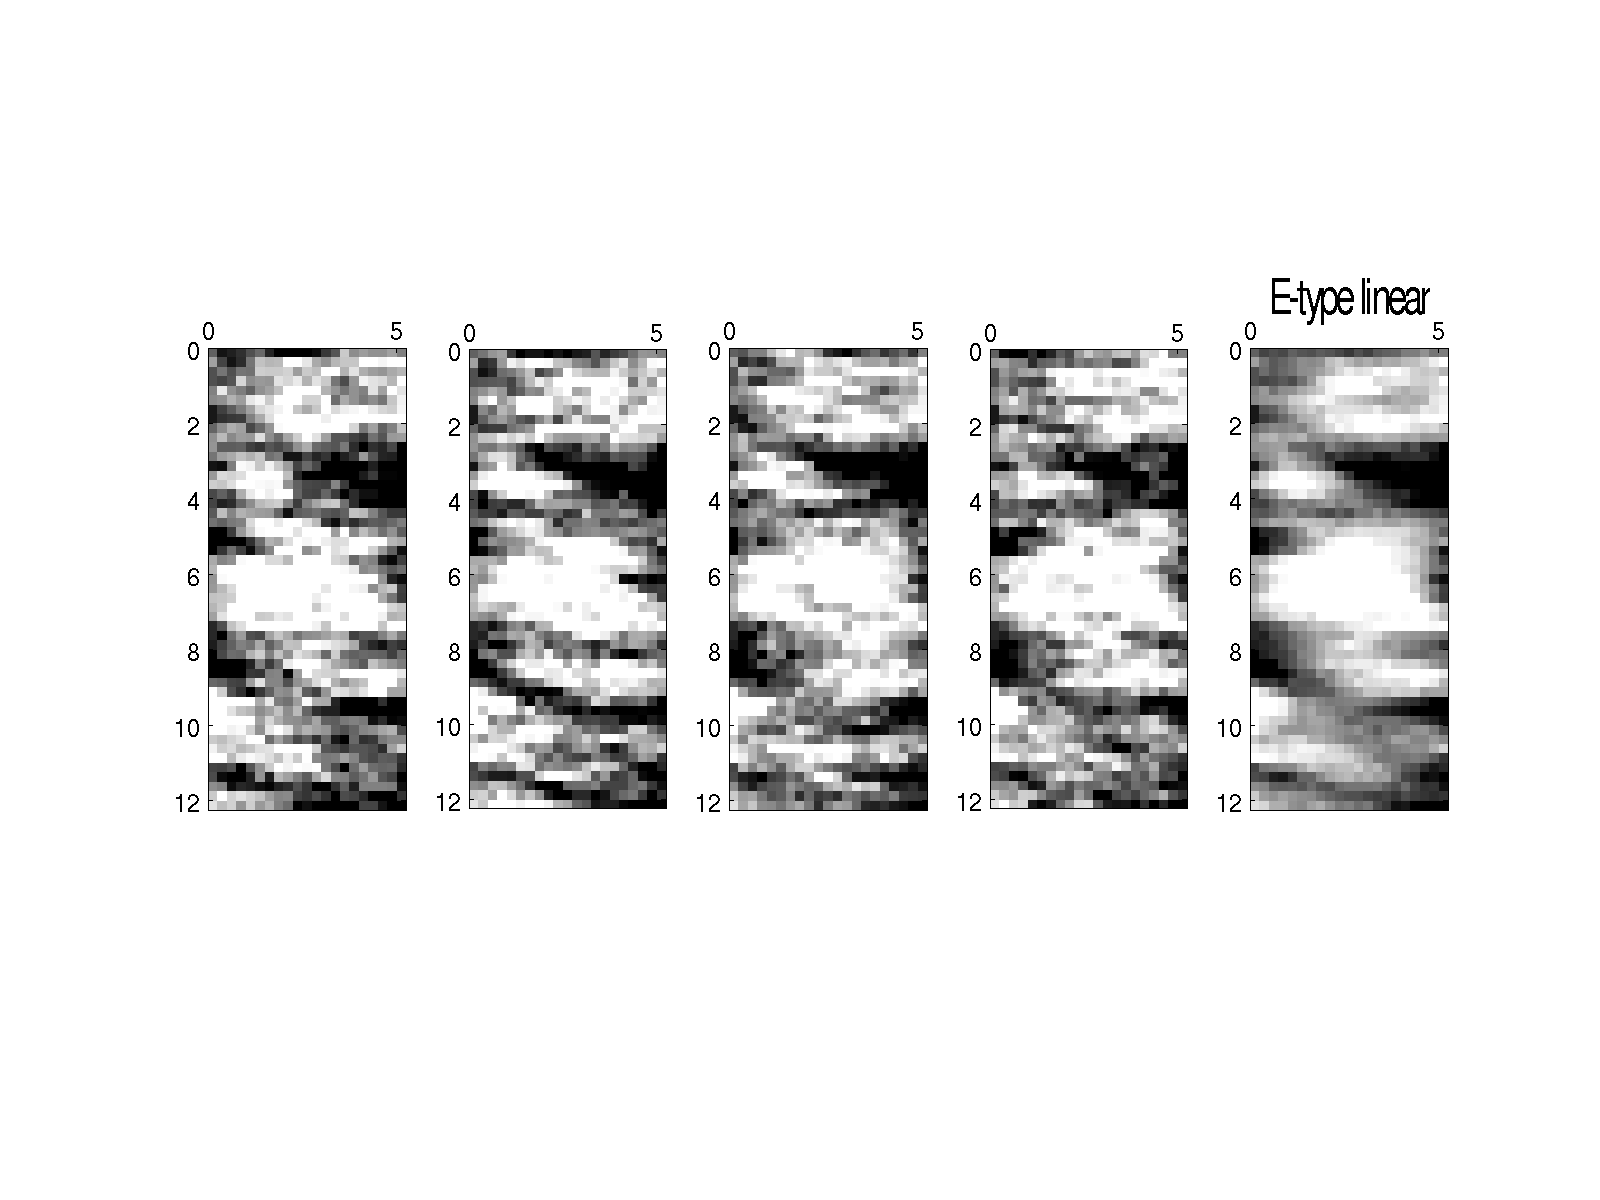
\includegraphics[width=14cm]{sim_lin}
  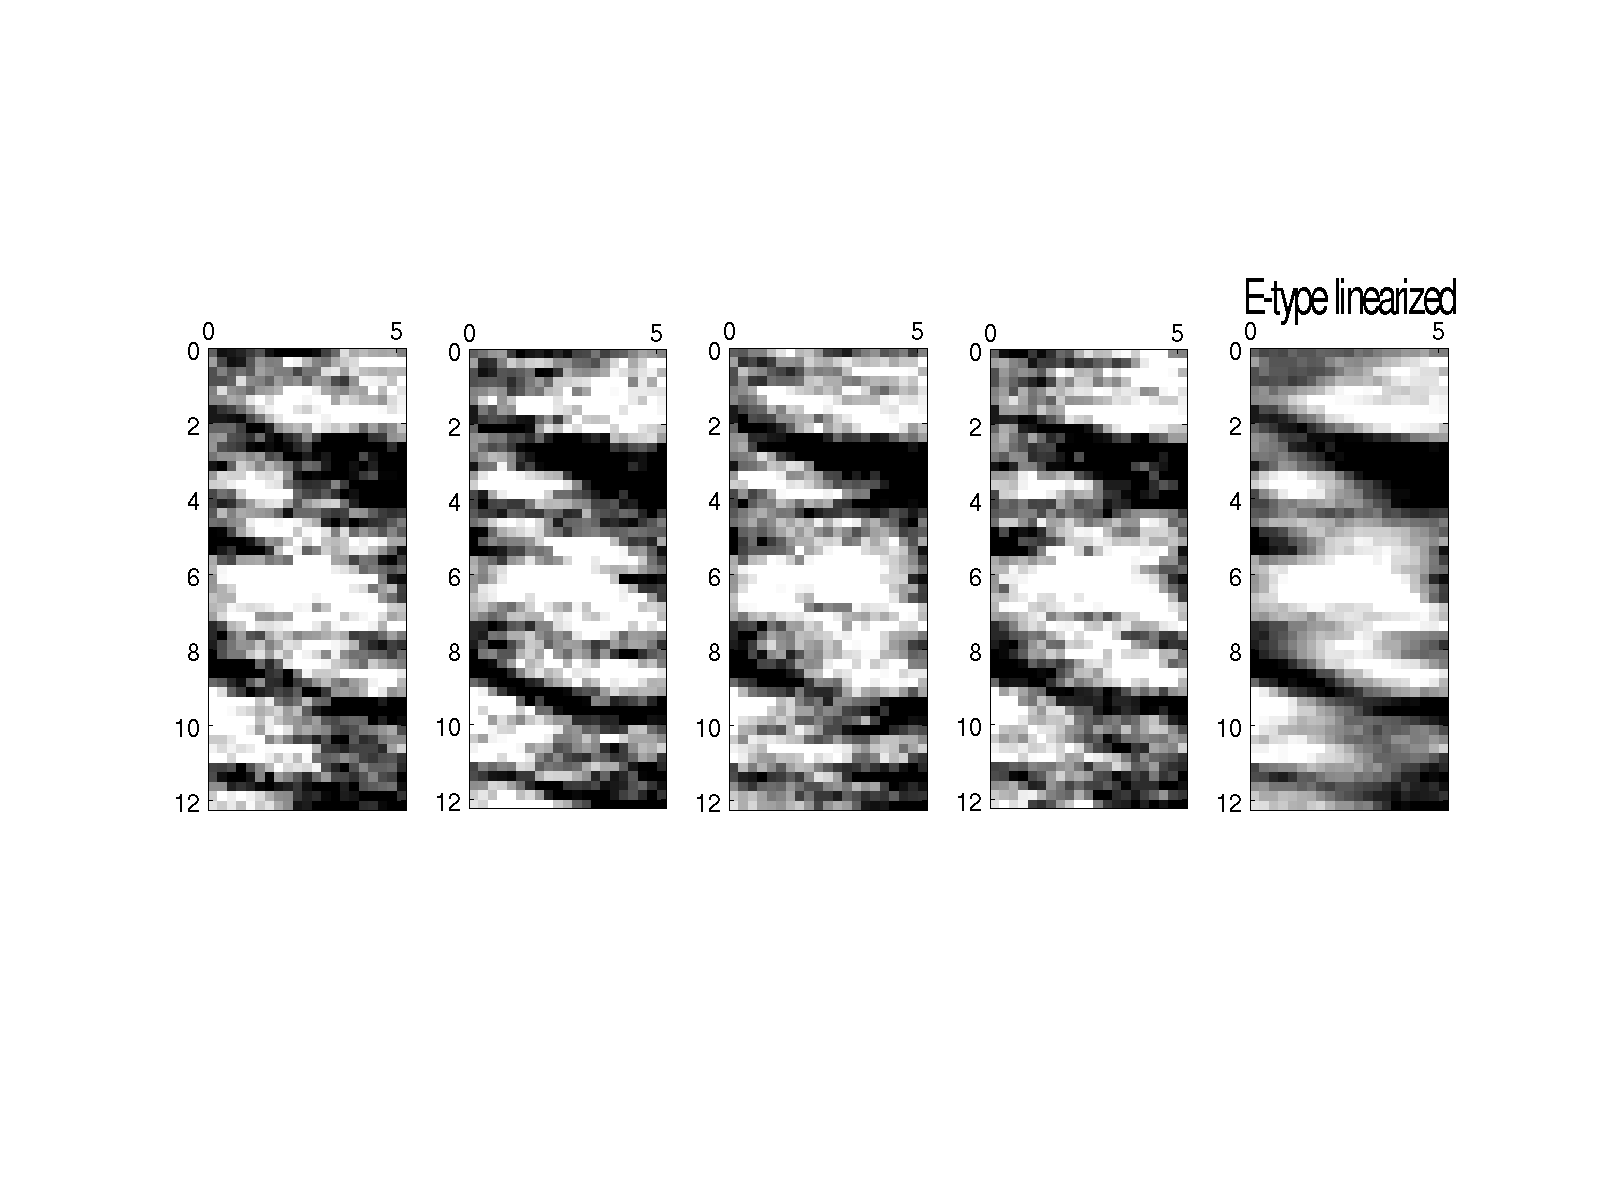
\includegraphics[width=14cm]{sim_iterative}
\caption[5 samples of the a posterior pdf using top) the true kernel, b) the constant velocity kernel, c) the linearized kernel.]{}
\label{fig:iterative_sim}
\end{figure}




\end{document}


